In this section, we'll discuss how to add Figures, Tables, and Citations to a \LaTeX\ document.
\subsection{Figures}
In \LaTeX, Figures and images are not the same thing.
Figures are an environment, while images represent their content (mostly).
This is actually very powerful,
since it allows you to combine multiple images, text, flow-charts, or whatever you like
in a single Figure.
\par
The Figure environment is invoked like equations: \lstinline|\begin{figure} ... \end{figure}|.
\par
To embed images, we need to use the \lstinline|graphicx| package,
and also tell it where to look for images using \lstinline|\graphicspath{{folder/},{anotherfolder/},...}|.
Then, we can use \lstinline|\includegraphics{imagename}| to add the image to the \lstinline|figure| environment.
\par
To caption the figure, we use the \lstinline|\caption{caption text}| command within the \lstinline|figure| environment,
which automatically numbers the Figure based on the document class.
\par
Just like equations, we can use \lstinline|\label{}| and \lstinline|\ref{}| to reference the Figure number elsewhere.
The nice part is, whenever Figures are moved around, \LaTeX\ takes care of the number ordering,
and the in-text references always point to the same Figure.
\par
Putting it all together:
\par
\textbf{Code:}
\begin{lstlisting}
  Figure \ref{fig:devs} shows Ballmer shortly after the peak.
  \begin{figure}[H]
    \centering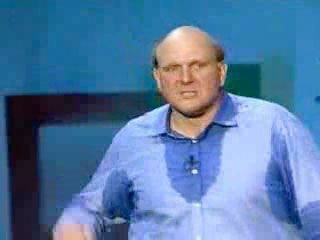
\includegraphics[width=0.5\textwidth]{developers.jpg}
    \caption{Developers}\label{fig:devs}
  \end{figure}
\end{lstlisting}
\textbf{Result:}
\par
Figure \ref{fig:devs} shows Ballmer shortly after the peak.
\begin{figure}[H]
  \centering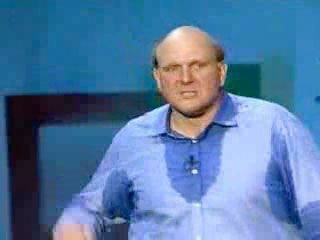
\includegraphics[width=0.5\textwidth]{developers.jpg}
  \caption{Developers}\label{fig:devs}
\end{figure}
\subsubsection{Extra Tips}
Its usually good to use \lstinline|\centering| before \lstinline|\includegraphics| to centre the image.
\par
The command \lstinline|\includegraphics| also accepts optional arguments for \lstinline|width=...|, \lstinline|height=...|, etc.
Best practice is to set this to \lstinline|0.5\textwidth|, or some proportion other than 0.5,
so that the image adapts to the margins.
Note that \lstinline|0.5*\textwidth| will give an error -- the multiplication of lengths is implicit.
\subsubsection{Tikz}
The \lstinline|tikz| package provides tools for creating flow-charts.
The flow-chart is written using \LaTeX\ code,
but best practice is to write the code in a separate file,
and then include the file using \lstinline|\include{filename}|.
\par
Figure~\ref{fig:structure} gives an example flow-chart (namely, the contents of this document).
The syntax of \lstinline|tikz| is essentially a language all of its own,
and we're not going to delve into it any further here.
In \ref{ap:code-tikz}~\nameref{ap:code-tikz}, you can see the code used to create Figure~\ref{fig:structure}.
\begin{figure}[H]
    \centering
    \tikzset{%
  arrow/.style    = { ->,
                      very thick,
                      rounded corners,
                      >     = Latex,
                      draw  = black!60!white },
  element/.style  = { very thick,
                      fill  = white,
                      draw  = #1!60!white,
                      align = center,
                      font  = \ttfamily },
}
\begin{tikzpicture}
  \node(main)  [element=red,fill=red!20!white]{main.tex};
  \node(config)[element=blue,left = 1cm of main]{config.tex};
  \node(cls)   [element=gray,above = 1cm of main]{mitthesis.cls};
  \draw[arrow] (config) -- (main);
  \draw[arrow] (cls) -- (main);
  
  \coordinate [above right = 1.75cm and 4cm of main] (files);
  \coordinate [right = 1cm of main] (fx);
  \foreach \i/\file in {
     0/front,
     1/contents,
     2/ch-intro,
     3/ch-math,
     4/ch-figs-tabs-cite,
     5/ch-conclusion,
     6/ap-links,
     7/ap-code%
   }{
      \node(\file) [element=blue,below = 0.7*\i cm of files]{\file.tex};
      \draw[arrow] (\file) -| (fx) -- (main);
  }
  \coordinate [above left = 2.45cm and 3cm of config] (files);
  \coordinate [left = 1cm of config] (fx);
  \coordinate [below = 3.55cm of fx] (xl);
  \foreach \i/\file in {
    0/tikz,
    1/hyperref,
    2/nameref,
    3/graphicx,
    4/amsmath,
    5/lstlistings,
    6/booktabs,
    7/float,
    8/biblatex%
  }{
      \node(\file) [element=green,below = 0.7*\i cm of files]{\file};
      \draw[arrow] (\file) -| (fx) -- (config);
  }
  \node(lib)[element=purple, below = 1.8cm of config] {library.bib};
  \draw[arrow] (lib) -- (config);
  \draw[arrow] (biblatex.south) |- (xl) -| (lib.south);
\end{tikzpicture}
    \caption{Overview of this document}
    \label{fig:structure}
\end{figure}
\subsection{Tables}
Tables are almost identical to Figures, except this time the content is a \lstinline|tabular| environment,
and the table object is a \lstinline|table| environment.
\par
You can specify the alignment of each column using the argument to a \lstinline|tabular| environment:\\
\lstinline|\begin{tabular}{lcr} ... \end{tabular}|, where \lstinline|lcr| defines 3 columns, having
\textbf{l}eft, \textbf{c}enter, and \textbf{r}ight alignment.
Within the table content,
rows are separated by newlines: \lstinline|\\|, while
columns are separated by the \lstinline|&| symbol.
Here is an example:
\par
\textbf{Code:}
\begin{lstlisting}
\begin{table}[H]
  \centering\caption{Windows Operating Systems}
  \vspace{0.5em}
  \begin{tabular}{ccl}\toprule
  	Year & OS & Reviews    \\ \midrule
  	2009 & 7  & a triumph  \\
  	2012 & 8  & a disaster \\
  	2016 & 10 & meh        \\ \bottomrule
  \end{tabular}
\end{table}
\end{lstlisting}
\textbf{Result:}
\begin{table}[H]
  \centering\caption{Windows Operating Systems}
  \vspace{0.5em}
  \begin{tabular}{ccl}\toprule
  	Year & OS & Reviews    \\ \midrule
  	2009 & 7  & a triumph  \\
  	2012 & 8  & a disaster \\
  	2016 & 10 & meh        \\ \bottomrule
  \end{tabular}
\end{table}
\subsection{Citations}
Automatically generating citations is another helpful feature of \LaTeX.
However, setting up the workflow can be a little tricky.
\par
First, you'll need a bibliography file. These can be exported from reference managers like
\href{https://mendeley.com}{Mendeley} or
\href{https://www.zotero.org/}{Zotero}.
In \ref{ap:code-bib}~\nameref{ap:code-bib} an example is given.
\par
\textbf{Code:}
\par
Within your document header, you need to load the package \lstinline|biblatex|
(with whichever formatting options suit you),
and specify your bibliography file: \lstinline|\bibliography{library.bib}|.
\par
Then, within the body of the document, you can use the \lstinline|\cite{...}| command to cite a reference,
replacing \lstinline|...| with the \lstinline|id| of the desired entry in your \lstinline|.bib| file
(e.g.\ \lstinline|Ashburner2005|).
\par
Finally, wherever you want the bibliography to appear, you can use the
\lstinline|\printbibliography| command.
\par
\textbf{Compiling:}
\par
We're not out of the woods yet.
The document compiler, \lstinline|latex|, doesn't actually do reference management.
There are several other tools which can do this (and actually, choosing one
\href{https://tex.stackexchange.com/questions/25701/}{gets complicated}).
A good choice here however, is \lstinline|bibtex|.
\par
What you need to do is:
compile your document with \lstinline|latex|,
then again with \lstinline|bibtex|,
and then one last time with \lstinline|latex| again.
For a document called \lstinline|main.tex|, this looks like:\\
\lstinline|  $ latex main|\\
\lstinline|  $ bibtex main|\\
\lstinline|  $ latex main|\\
What happens is:
\lstinline|latex| compiles the document as much as possible,
putting placeholders for every citation,
and producing a list of the missing references (and formatting specifications)
in an auxiliary file (\lstinline|main.aux|);
\lstinline|bibtex| then looks for \lstinline|main.aux|,
and uses the specifications and bibliography file to create one more file, \lstinline|main.bbl|,
which provides \lstinline|latex| with formatted answers for each of the citation placeholders;
the second pass of \lstinline|latex| then finds \lstinline|main.bbl| and replaces
the placeholders (including the bibliography itself) with the formatted citation information.
\par
\subsubsection{Example}
\textbf{Code:}
\par
\begin{lstlisting}
  Unified Segmentation by \citeauthor{Ashburner2005} (\citeyear{Ashburner2005})
  is a popular model for segmenting brain MRI \cite{Ashburner2005}.
  \par
  \subsubsection*{References}
  \bibliography{refs.bib}
\end{lstlisting}
\textbf{Result:}
\par
Unified Segmentation by \citeauthor{Ashburner2005} (\citeyear{Ashburner2005})
is a popular model for segmenting brain MRI \cite{Ashburner2005}.
\par
\subsubsection*{References}
\bibliography{refs.bib}
